\chapter{Theory}
\label{c:theory}
\vspace{0.6cm}
In this chapter the standard model (SM) of particle physics is introduced, including QED, weak and QCD interactions. A brief description of the theory of proton-proton collisions is given before a discussion of the physics of the top quark, including four-top-quark production. Some of the shortcomings of the SM are described, after which a discussion of some of the models beyond the standard model (BSM) which can produce four-top-quark signatures is presented. The concepts of `effective field theories' and `simplified models' are introduced.

\section{Standard Model}

The SM~\cite{Glashow:1961tr,PhysRevLett.19.1264,Salam:1968rm,DGriff} is a theory which describes the elementary particles and their interactions. Matter consists of six quarks and six leptons, each of which has an anti-particle with the same mass and opposite-sign charge. They are organised into three generations, each of which contains heavier particles than the last, as seen in Table~\ref{table:SMmatter}. All of the normal matter on Earth is made up of particles from the first generation, i.e.~up and down quarks make up protons and neutrons, and combined with electrons they form atoms. 

The leptonic sector consists of charged leptons, which can interact via the electromagnetic and weak forces, and neutrinos, which interact via the weak force only. The neutrinos are assumed to be massless in the SM, however, observations of neutrino oscillations have revealed that neutrinos have mass~\cite{PhysRevC.88.025501}.

\vspace{0.8cm}
\begin{table}[ht!]
\centering
\footnotesize
\begin{tabular}{|c|l|l|l|l|l|l|}
\hline
\multirow{2}{*}{Generation} & \multicolumn{3}{c|}{Quarks}                             & \multicolumn{3}{c|}{Leptons}              \\ \cline{2-7} 
                            & Flavour & Electric & Mass (MeV)                           & Flavour      & Electric & Mass (MeV)        \\
                            & & Charge &                            &       & Charge &         \\ \hline

\hline

\multirow{2}{*}{I}          & u       & 2/3    & $2.2^{+0.6}_{-0.4}$                  & e            & -1     & 0.511             \\
                            & d       & -1/3   & $4.7^{+0.5}_{-0.4}$                  & $\nu_{e}$    & 0      & $<2\times10^{-6}$ \\ \hline
\multirow{2}{*}{II}         & c       & 2/3    & $(1.27\pm 0.03)\times10^{3}$         & $\mu$        & -1     & 105.66            \\
                            & s       & -1/3   & $96^{+8}_{-4}$                       & $\nu_{\mu}$  & 0      & $<0.19$           \\ \hline
\multirow{2}{*}{III}        & t       & 2/3    & $(173.21\pm0.51\pm0.71)\times10^{3}$ & $\tau$       & -1     & $1776.86\pm0.12$  \\
                            & b       & -1/3   & $(4.18^{+0.04}_{-0.3})\times10^{3}$  & $\nu_{\tau}$ & 0      & $<18.2$           \\ \hline
\end{tabular}
\caption{The quarks and leptons in the SM~\cite{PDG2016}.}
\label{table:SMmatter}

\end{table}
Quarks interact via the electromagnetic, weak or strong forces. Each quark has an electric charge, as seen in Table~\ref{table:SMmatter}, and carries a colour charge of red, green or blue, where all three colours combined can form a colour-singlet state. A combination of quarks with a colour and its anti-colour can also form a colour-singlet state. The phenomenon of colour confinement means that quarks can only be found in colour-singlet states such as in baryons or mesons. 

Finally, the force carriers consist of gauge bosons of integer spin, as seen in Table~\ref{table:SMbosons}. Photons and Z bosons mediate neutral electroweak interactions whereas the W bosons mediate charged electroweak interactions. The gluons mediate the strong interaction and occur with 8 different types of colour charge which will be described in Section~\ref{subsec:QCD}. 
% The Graviton is hypothesised to carry the gravitational force but there is as yet no evidence to support this hypothesis.
\begin{table}[ht!]
\centering
\footnotesize
\begin{tabular}{|l|l|l|l|l|l|}
\hline
Gauge boson                       & Force           & Electric Charge & Mass (GeV) & Spin & Range (m)  \\ \hline \hline
Photon ($\gamma$)                 & electromagnetic & 0      & 0          & 1    & $\infty$   \\ \hline
W$^{\pm}$                         & weak            & $\pm1$ & $80.385\pm0.015$           & 1    & $10^{-18}$ \\ \hline
Z                                 & weak            & 0      & $91.1876\pm0.0021$           & 1    & $10^{-18}$ \\ \hline
gluon (g)                            & strong          & 0      & 0          & 1    & $10^{-15}$ \\ \hline
% Graviton\footnote{hypothesised} & gravitational   & 0      & 0          & 2    & $\infty$   \\ \hline
\end{tabular}
\caption{The gauge bosons of the SM~\cite{PDG2016}.}
\label{table:SMbosons}
\end{table}

The discovery of the Higgs boson in 2012~\cite{Higgs2012observation,Aad:2012tfa,Aad:2015zhl} completed the SM with an explanation of how the fundamental particles acquire mass via the electroweak symmetry breaking mechanism.

The SM is a gauge theory based on the symmetry group SU(3)$\times$SU(2)$\times$U(1), which is a combination of the electroweak interactions based on the SU(2)$\times$U(1) symmetry group and the strong interaction which is based on the SU(3) group.

In the following, the SM will be described in more detail.

\subsection{The gauge principle}
Emmy Noether showed that conservation laws result from underlying continuous symmetries of a physical system~\cite{Emmy}. This principle had a profound impact in the development of quantum field theories. A quantum field possesses gauge symmetries, where the gauge regulates the degrees of freedom of the Lagrangian. For the action of a system to be conserved, a Lagrangian should be invariant under continuous local gauge transformations (i.e. transformations that depend on the space-time point). Each group of transformations has one or more generators, each with an associated gauge (vector) field. Gauge bosons are quantisations of these gauge fields. Global transformations are a subset of local transformations where the transformation is not dependent on the space-time point.

\subsection{Electroweak theory}

\subsubsection{Quantum Electrodynamics}
\label{subsec:QED}

Quantum Electrodynamics is an Abelian gauge theory based on the U(1)$_{\textrm{EM}}$ symmetry group, which has the electric charge, q, as its generator. Figure~\ref{fig:QEDvertex} shows the elementary QED vertex where a charged particle (charged lepton or quark) and its anti-particle interact with a photon. The convention used in this thesis is that time flows from left to right. However, these diagrams may be rotated as long as they conserve energy. Hence, this vertex can describe particle-anti-particle annihilation into a photon, a photon pair-producing a particle-anti-particle pair, a particle emitting a photon or an anti-particle emitting a photon, depending on the orientation of the diagram. QED interactions conserve lepton or quark flavour.


\begin{figure}[ht!]
\begin{center}
    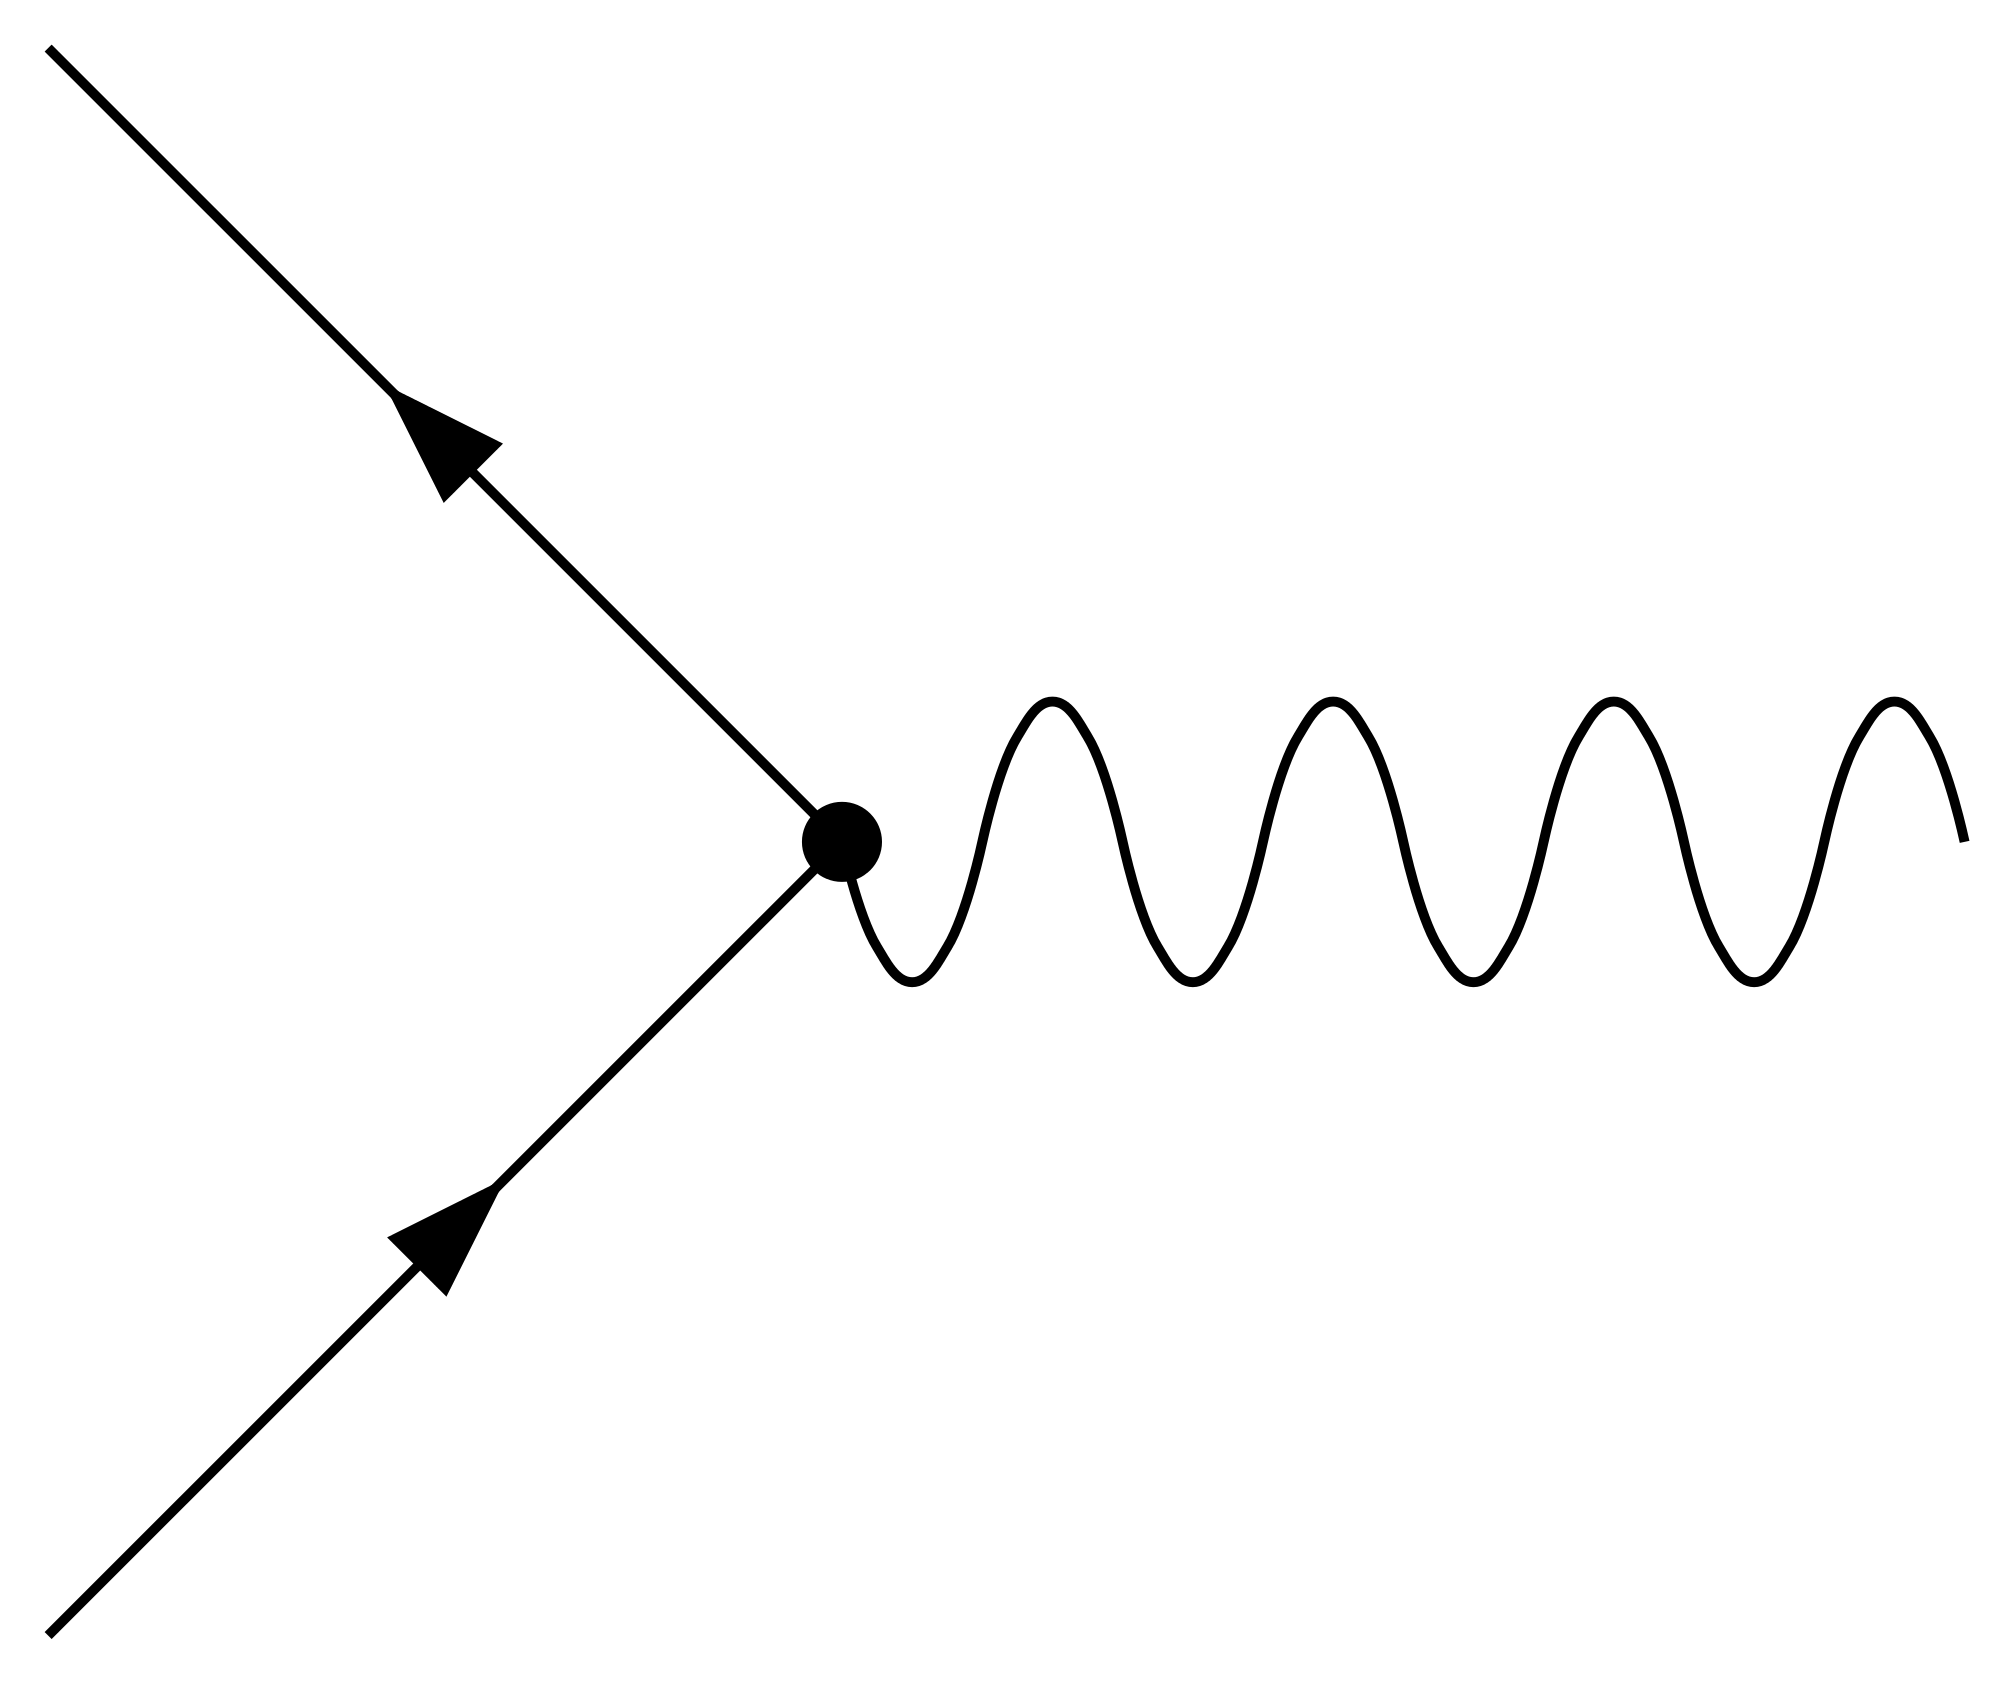
\includegraphics[width=0.35\textwidth]{images/Theory/QEDvertex.png}
    \caption{Elementary QED vertex.}
    \label{fig:QEDvertex}
\end{center}
\end{figure}

Feynman diagrams are visual representations of the terms in a perturbative series expansion with respect to the interaction strength around the non-interacting Lagrangian. Incoming particles are considered to be free particles, the interaction term then turns on and the outgoing particle are again considered to be free particles. Terms involving three or more fields represent interactions between the fields, and are referred to as vertex factors. The propagators can be described from the free particle Lagrangian and they represent intermediate states which connect vertices. Feynman diagrams are said to be at ``tree level'' if they are the representation of the leading order term in the expansion.\\
% Vertex factors are the elements of the Lagrangian of order three or higher which represent the interactions between fields. 
% This diagram alone cannot occur as it violates conservation of energy but it can be used to build a full Feynman diagram for a particle physics process.
The QED Lagrangian can be found in Eq.~\ref{eqn:QEDL} with $\psi$ representing a relativistic spin-1/2 field and $D_{\mu}$ representing the covariant derivative, which is defined as $D_{\mu} = \partial_{\mu} + iqA_{\mu}$. Here $q$ represents the charge of the particle and $A^{\mu}$ is the massless field of the electromagnetic four-potential. The mass of the particle is represented by $m$ and $F_{\mu\nu} = \partial_{\mu}A_{\nu} - \partial_{\nu}A_{\mu}$ is the electromagnetic field (or Faraday) tensor.

\begin{equation}
\mathcal{L} = \overline{\psi}\left(i\gamma^{\mu}D_{\mu}-m\right)\psi - \frac{1}{4}F_{\mu\nu}F^{\mu\nu}
\label{eqn:QEDL}
\end{equation}

The Dirac Lagrangian is manifestly invariant to global phase transformations $\psi \rightarrow e^{i\theta} \psi$. The supplementation by $iqA_{\mu}$ is required to make the Lagrangian invariant to local phase transformations $\psi \rightarrow e^{i\theta(x)} \psi$ where $A_{\mu}$ transforms as $A_{\mu} \rightarrow A_{\mu} - \frac{1}{q} \partial_{\mu}\theta(x)$. Hence, the QED Lagrangian is gauge invariant under U(1) phase transformations, where U(1) is the unitary group of complex numbers. 


Application of the Euler-Lagrange equations to Eq.~\ref{eqn:QEDL} leads to the derivation of the Dirac Equation shown in Eq.~\ref{Eqn:Dirac}.
% , where $J_{\mu} = \overline{\psi}\gamma_{\mu}\psi$.

% \begin{equation}
% \left( \gamma^{\mu }\partial _{\mu } -m - iq\gamma^{\mu }A_{\mu}\right)\psi = 0
% \label{Eqn:Dirac}
% \end{equation}

\begin{equation}
\left( i\gamma^{\mu} D_{\mu} - m \right)\psi = 0
\label{Eqn:Dirac}
\end{equation}


The Dirac equation describes the motion for spin-1/2 particles with mass, ie. quarks and charged leptons.


 % From this equation the Feynman rules for QED can be derived. These rules allow the computation of a number, known as the \emph{amplitude}, for each Feynman diagram. The sum total of the amplitudes for all diagrams which represent a particular process can be summed to produce the probability or \emph{cross section} for that process to occur.

In QED the vacuum acts like a dielectric medium which produces electron-positron pairs where the virtual electron is attracted to positive charges and the virtual positron is repelled (and vice versa for negative charges). This vacuum polarisation partially screens the charged particle and effectively reduces its field. However at short distances, the effective charge increases as the screening reduces.
% \textbf{Effective coupling}

\subsubsection{Weak interactions}

The charged weak interaction is the only interaction where a flavour changing process can occur. There are two W bosons, one of positive charge and one of negative charge, W$^{\pm}$. The diagram of weak nuclear decay in Fig.~\ref{fig:QEDvertex} illustrates the W boson's interaction with different flavour quarks and leptons.


\begin{figure}[ht!]
\begin{center}
    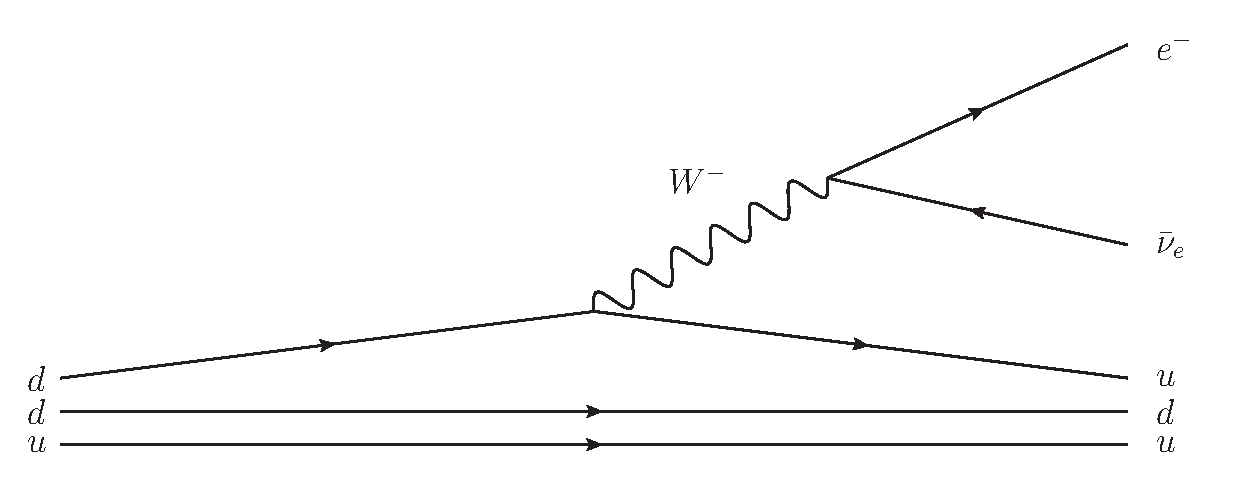
\includegraphics[width=0.65\textwidth]{images/Theory/weakDecay2.eps}
    \caption{Weak nuclear decay of neutron to proton.}
    \label{fig:QEDvertex}
\end{center}
\end{figure}

The neutral weak interaction is mediated by Z bosons which can interact with any quark or lepton as long as the flavour is conserved at the vertex.

% As the weak force bosons are massive, this means that weak decays are much slower than decays via electromagnetism for instance. This means that particles that can only decay via the weak force have longer lifetimes. 
The weak force only interacts with chirality left-handed (right-handed) particles (anti-particles).
% , ie. particles where the spin is (anti-)aligned with the momentum direction. 
The charge for weak interaction is \emph{weak isospin} ($I_{3}$) which is $\pm1/2$ for left-handed fermions, $\pm1$ for W$^{\pm}$, and zero otherwise.

Weak interactions are the only interactions known to violate parity conservation, which was hypothesised by Yang and Lee~\cite{PhysRev.104.254} and experimentally validated by Wu in 1957~\cite{PhysRev.105.1413}. It was later discovered that weak interactions also violate the combined charge-parity (CP) symmetry~\cite{Cronin2012,PhysRevLett.13.138}.


\subsubsection{Electroweak Unification}

Glashow~\cite{Glashow:1961tr}, Weinberg~\cite{PhysRevLett.19.1264} and Salam~\cite{Salam:1968rm} formulated the unification of the weak and electromagnetic forces combined in the SU(2)$_{\textrm{L}}$~x~U(1)$_{\textrm{Y}}$ gauge group. They are hypothesised to merge into one electroweak force above the unification energy of $\approx 100$~GeV. Weak hypercharge is defined as $Y_{W} = 2(q-I_{3})$. $Y_W$ is the generator of the U(1)$_{\textrm{Y}}$ component of the electroweak gauge group, which is mediated by the B boson. In the SU(2)$_{\textrm{L}}$ component of the electroweak theory, the left-handed fields transform as doublets and the right-handed fields transform as singlets. It is only in the weak interaction that left-handed and right-handed particles are treated differently. The generators of the SU(2)$_{\textrm{L}}$ component are ${\bf T} = \boldsymbol{\sigma}/2$ where $\boldsymbol{\sigma}$ are the Pauli matrices.
The left-handed doublet, $\psi_L$, can consist of either a left-handed up-type and a left-handed down-type quark, or a left-handed neutrino and left-handed charged lepton. The right-handed field, $\psi_R$, can be either a right-handed up-type quark, a right-handed down-type quark, or a right-handed charged lepton. Right-handed neutrinos have not been observed. The possible left-handed and right-handed fields are:

\begin{equation*}
\psi_L = \twovector{u_L}{d_L}, \twovector{\nu_L}{\ell_L}~~~~\psi_R=~u_R,~d_R,~\ell_R
\end{equation*}
where $u_L$ and $d_L$ represent all up-type and down-type quarks, respectively.

The projection operators, $\textrm{P}_{L/R}=\frac{1}{2}(1\pm\gamma^{5})$, are used to obtain the left-handed and right-handed components of fermionic fields via:
\begin{equation}
\psi = \textrm{P}_{L}\psi + \textrm{P}_{R}\psi = \psi_{L} + \psi_{R}
\end{equation}

where $\gamma_{5}$ is a combination of the gamma matrices:
\begin{equation}
\gamma_{5} = i\gamma_{0}\gamma_{1}\gamma_{2}\gamma_{3} = 
{\begin{pmatrix}
0&I_{2}\\
I_{2}&0
\end{pmatrix}}
\end{equation}

To ensure local gauge invariance, the covariant derivative is defined as:
\begin{equation}
D_{\mu} = \partial_\mu  + i g \mathbf{T} \cdot \mathbf{W}_{\mu} + i \frac{g'}{2} Y_{W} B_\mu
\label{eqn:EQcov}
\end{equation}
Here four new gauge fields are introduced. The triplet of fields $\mathbf{W} = W^{a}~(a=1,~2,~3)$ are required for SU(2)$_{\textrm{L}}$ gauge invariance with coupling constant $g$, and the gauge field B$_{\mu}$ is required for U(1)$_{\textrm{Y}}$ gauge invariance with coupling constant $g'$. For right-handed singlet particles, $\mathbf{T}=\mathbf{0}$ and the second term in Eq.~\ref{eqn:EQcov} vanishes.
% The theory contains four gauge bosons: three W bosons W$_{a}~(a=1,~2,~3)$ and one B boson.
Equation~\ref{eq:EWK_L} shows the Lagrangian for electroweak interactions, where $\mathbf{W}_{\mu\nu}^{a}$ and $B_{\mu\nu}$ are the field strength tensors for the  $W^{a}_{\mu}$ and $B_{\mu}$ fields, respectively.
% \begin{equation}
% \label{eq:EWK_L}
% \begin{split}
% \calL_\textrm{EWK} & = \bar{\psi}_L \gamma^\mu ( i\partial_\mu  - g \mathbf{T} \cdot \mathbf{W}_\mu - \frac{g'}{2} Y_{W}
% B_\mu) \psi_L \\ & + \bar{\psi}_R \gamma^\mu (i \partial_\mu - \frac{g'}{2} Y_{W} B_\mu) \psi_R \\& 
% -\frac{1}{4}\mathbf{W}_{\mu\nu}^{a} \mathbf{W}^{\mu\nu}_{a} -\frac{1}{4}B_{\mu\nu} B^{\mu\nu}
% \end{split}
% \end{equation}

% \begin{equation}
% \label{eq:EWK_L}
% \calL_\textrm{EWK}  = \bar{\psi}_L i \gamma^\mu D_\mu  \psi_L + \bar{\psi}_R i \gamma^\mu D_\mu  \psi_R 
%  - \frac{1}{4}\mathbf{W}_{\mu\nu}^{a} \mathbf{W}^{\mu\nu}_{a}  -\frac{1}{4}B_{\mu\nu} B^{\mu\nu}
% \end{equation}

\begin{equation}
\label{eq:EWK_L}
\calL_\textrm{EWK}  = \bar{\psi} i \gamma^\mu D_\mu  \psi - \frac{1}{4}\mathbf{W}_{\mu\nu}^{a} \mathbf{W}^{\mu\nu}_{a}  -\frac{1}{4}B_{\mu\nu} B^{\mu\nu}
\end{equation}

% It can be seen that the left-handed fermion fields, $\psi_{L}$, couple to the W and B bosons and the right-handed fermion fields, $\psi_{R}$, couple to the B boson only. 

The fields of the four more familiar physical gauge bosons from Table~\ref{table:SMbosons}, $W^{\mu\pm}$, $Z^{\mu}$ and the photon ($A^{\mu}$), are linear combinations of the gauge fields ${W}_{\mu}^{a}$ and $B_\mu$. This is represented in Eqs.~\ref{eqn:Zgamma} \&~\ref{eqn:Wpm}, where $\theta_{W}$ is the weak mixing angle.
\begin{equation}
\label{eqn:Zgamma}
{\begin{pmatrix}
A^{\mu} \\
{Z^{\mu}} 
\end{pmatrix}}
=
{\begin{pmatrix}
\cos\theta_{W} & \sin\theta_{W} \\
-\sin\theta_{W} & \cos\theta_{W} 
\end{pmatrix}}
{\begin{pmatrix}
{B}^{\mu} \\
{W}_{3}^{\mu}
\end{pmatrix}}
\end{equation}

\begin{equation}
\label{eqn:Wpm}
\textrm{W}^{\mu\pm}=\frac{1}{\sqrt{2}}\left(\textrm{W}_{1}^{\mu} \mp i\textrm{W}_{2}^{\mu}\right)
\end{equation}

% Equation~\ref{eqn:EWL} shows the electroweak Lagrangian where $\mathcal{L}_{K}$ gives the kinetic term, $\mathcal{L}_{N}$ gives the neutral interactions and $\mathcal{L}_{C}$ the charged interactions. $\mathcal{L}_{H}$ gives the Higgs three and four point self-interactions and  $\mathcal{L}_{HV}$ gives the Higgs interactions for vector bosons.  $\mathcal{L}_{WWV}$ ($\mathcal{L}_{WWVV}$) gives the three (four) point interactions of the vector bosons and $\mathcal{L}_{Y}$ gives the Yukawa couplings between the Higgs field and the fermions.

% \begin{equation}
% \label{eqn:EWL}
% \mathcal{L}_{EW} = \mathcal{L}_{K} + \mathcal{L}_{N} + \mathcal{L}_{C} + \mathcal{L}_{H} + \mathcal{L}_{HV} + \mathcal{L}_{WWV} + \mathcal{L}_{WWVV} + \mathcal{L}_{Y}
% \end{equation}

% and $\psi_L$ and $\psi_R$ are summed over all possibilities shown in Equations~\ref{eq:lepton_EWK_fields} and
% \ref{eq:quark_EWK_fields}.

% The Yukawa couplings, which describe the couplings between dirac fields and a scalar field, 
The spontaneous symmetry breaking mechanism proposed by Brout, Englert~\cite{PhysRevLett.13.321} and Higgs~\cite{PhysRevLett.13.508} results in the Higgs field getting a vacuum expectation value (VEV) and the electroweak Lagrangian changing form as described in Ref~\cite{Pich:2005mk}. It now has a kinetic term, a term for the neutral interactions and one for the charged interactions. Also introduced is a term for the Higgs three and four point self-interactions and another term for the Higgs interactions with vector bosons. There is a term for both the three and four point interactions of the vector bosons and another term for the Yukawa couplings between the Higgs field and the fermions.  It is through the spontaneous symmetry breaking mechanism that the W$^{\pm}$ and Z bosons gain mass. Fermions also acquire mass due to Yukawa terms as shown in Eq.~\ref{eqn:yukawaMass}. Here $M_f$ is the mass of the fermion, $Y_f$ is the Yukawa coupling and $v$ is the vacuum expectation value.

\begin{equation}
M_f = Y_f \frac{v}{\sqrt{2}}
\label{eqn:yukawaMass}
\end{equation}
% \begin{equation}
% \label{eqn:EWL2}
% \mathcal{L}_{EW} = \mathcal{L}_{K} + \mathcal{L}_{N} + \mathcal{L}_{C} + \mathcal{L}_{H} + \mathcal{L}_{HV} + \mathcal{L}_{WWV} + \mathcal{L}_{WWVV} + \mathcal{L}_{Y}
% \end{equation}

The charged current interaction is particularly interesting for the W decays from top quarks. It is described by the term in Eq.~\ref{eqn:CCint}, where $\psi_L$ is now rotated from flavour eigenstate to the weak eigenstate,.

\begin{equation}
\label{eqn:CCint}
\mathcal{L}_{C} = \frac{g}{\sqrt{2}} i\bar{\psi_{L}} \gamma^{\mu} \partial_{\mu} \psi_{L}
\end{equation}
\begin{equation*}
\psi_L = \twovector{u_L}{{d'}_L}, \twovector{\nu_L}{l_L}
\end{equation*}

The weak eigenstates are related to the flavour eigenstates through the CKM matrix, $V_{CKM}$, via ${d^{\prime}}_L = V_{CKM}~d_L$, where ${d^{\prime}}_L$ is a superposition of the flavour eigenstates. The CKM matrix, also known as the \emph{quark mixing matrix}, is a unitary matrix which describes the strength of the couplings for weak decays, as shown in Eq.~\ref{eqn:CKM1}. 
\begin{equation}
\label{eqn:CKM1}
{\begin{pmatrix}
d^{\prime }\\
s^{\prime }\\
b^{\prime }
\end{pmatrix}}
=
{\begin{pmatrix}
V_{ud}&V_{us}&V_{ub}\\
V_{cd}&V_{cs}&V_{cb}\\
V_{td}&V_{ts}&V_{tb}
\end{pmatrix}}
{\begin{pmatrix}d\\s\\b
\end{pmatrix}}
\end{equation}
The amplitudes for the up-type quarks to transition to down-type quarks are given in Eq.~\ref{eqn:CKM2}~\cite{PDG2016}.
\begin{equation}
\label{eqn:CKM2}
{\begin{pmatrix}
|V_{ud}|&|V_{us}|&|V_{ub}|\\|V_{cd}|&|V_{cs}|&|V_{cb}|\\|V_{td}|&|V_{ts}|&|V_{tb}|
\end{pmatrix}}
=
{\begin{pmatrix}0.97417\pm 0.00021 & 0.2248\pm 0.0006 & 0.00409\pm{0.00039}\\
0.220\pm 0.005 & 0.995\pm 0.016 & 0.0405\pm{0.0015}\\
0.0082\pm{0.0006} & 0.040\pm{0.0027}&1.009\pm0.031
\end{pmatrix}}
\end{equation}





\subsection{Quantum chromodynamics}

Quantum chromodynamics (QCD) is a non-Abelian gauge theory based on the SU(3)$_{C}$ symmetry group that describes the strong interactions between quarks and gluons. Quarks and gluons carry colour charge, $C$. Each (anti-)quark will carry one of (anti-)~red, (anti-)~green or (anti-)~blue colour charge whilst there are 8 types of gluon which exist in a superposition of colour-anti-colour states. One of the elementary QCD vertices is shown in Fig~\ref{fig:QCDvertex} where two quarks couple to a gluon. There are also three and four-point interactions between gluons.
\label{subsec:QCD}
\begin{figure}[ht!]
\begin{center}
    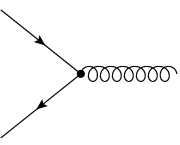
\includegraphics[width=0.35\textwidth]{images/Theory/QCDvertex.png}
    \caption{An elementary QCD vertex.}
    \label{fig:QCDvertex}
\end{center}
\end{figure}

The Gell-Mann matrices, $\lambda_{\alpha}$, are the generators of the SU(3)$_{C}$ group. In QCD, the covariant derivative is $D_{\mu} = \partial_{\mu} - i g A^{\alpha}_{\mu} \lambda_{\alpha}$ where $g$ represents the strong coupling constant and $A^{\alpha}_{\mu}$ represents the gluon field.
Equation~\ref{eqn:QCDL} gives the QCD lagrangian, $\mathcal{L}_{\textrm {QCD}}$ , where $G_{\mu \nu }^{a}=\partial _{\mu }{\mathcal {A}}_{\nu }^{a}-\partial _{\nu }{\mathcal {A}}_{\mu }^{a}+gf^{abc}{\mathcal {A}}_{\mu }^{b}{\mathcal {A}}_{\nu }^{c}$ is the gluon field strength tensor and $f^{abc}$ are the structure constants of SU(3). 
\begin{equation}
    \label{eqn:QCDL}
{\mathcal {L}}_{\mathrm {QCD} }={\bar {\psi }}_{i}\left(i(\gamma ^{\mu }D_{\mu })_{ij}-m\,\delta _{ij}\right)\psi _{j}-{\frac {1}{4}}G_{\mu \nu }^{a}G_{a}^{\mu \nu }
\end{equation}

\textbf{Asymptotic freedom and colour confinement}\\
Quark-anti-quark loops lead to screening of the quark colour charge, however gluon loops contribute the opposite by `anti-screening'. It was found that in any theory with $11n>2f$, where $n$ is the number of ``colours'' and $f$ is the number of ``quark flavours'', the coupling constant, $\alpha_{S}\left( |q^{2}| \right)$, will decrease with increasing energy, q$^{2}$~\cite{PhysRevLett.30.1343,PhysRevLett.30.1346}. This is known as \emph{asymptotic freedom} as the quarks inside hadrons effectively act like free particles. This is in contrast to QED where there is no `anti-screening' effect.

% \begin{equation}
% \label{eqn:alphaSQCD}
% \alpha_{S}\left( |q^{2}| \right) = \frac{\alpha_{S}\left( \mu^{2} \right)} {1 + \left[ \alpha_{S}\left( \mu^{2} \right)/12\pi \right]\left( 11n -2f \right) \ln \left(|q^{2}|/\mu^{2}\right)}
% \end{equation}

With increasing spatial separation, the strong force increases. Energy which has gone into separating two quarks reaches a critical point (at a distance of $\approx 1$~fm) where it is transferred into producing more quarks which accompany the separated quarks to form hadrons. This cascade of separated quarks, or parton shower, into hadrons is called \emph{hadronisation}. This is the principle of \emph{confinement} and it is the reason that colour doublets or octets are never found in nature, only colour singlet states such as mesons and baryons. This is in contrast, again, to QED where free particles can carry electric charge.


\section{Proton-proton collisions}
% At a lepton collider, one can assume that the initial particles involved in a collision are fundamental particles which means precise details of the initial state are known. However 
At the Large Hadron Collider (LHC) the particles involved in the collisions are protons\footnote{There are also collisions with lead ions but they are not considered in this thesis.}, which are complex composite particles consisting of three valence quarks (two up quarks and one down quark) and gluons which exchange the strong force. The proton also contains `sea quarks' which are quark-anti-quark pairs that come into and out of existence rapidly and continuously within the proton due to gluon colour field splitting.

Figure~\ref{fig:protonPDF} shows the parton distribution functions for the proton. These are interpreted as the probability for a quark to be carrying a fraction, $x$, of the proton's momentum in the longitudinal direction.

\begin{figure}[ht!]
\begin{center}
    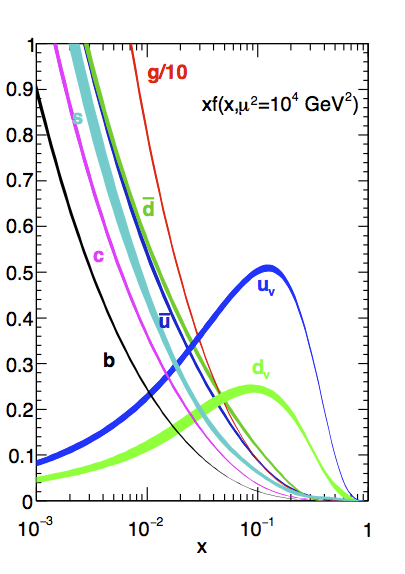
\includegraphics[width=0.6\textwidth]{images/Theory/pdfnob.png}
    \caption{Proton parton distribution functions $xf(x)$ $(f = u_{v},~ d_{v},~ \overline{u},~ \overline{d},~ s\approx\overline{s},~ c\approx\overline{c},~ b\approx\overline{b},~ g$ ) for a given momentum fraction, $x$. The fermions are considered to be sea quarks except in the case of $u_{v}$ and $d_{v}$, which are valence quarks. The gluon contribution has been scaled by a factor of ten for visibility. Obtained from NNLO NNPDF3.0~\cite{Ball2015}.}
    \label{fig:protonPDF}
\end{center}
\end{figure}

Protons in the LHC may a) not interact at all and continue to be accelerated around the ring, b) interact via a soft scatter where the products mostly travel along the direction of the beam, c) participate in a hard interaction where two partons within the protons have a high energy collision in which the products travel transverse to the beam. In the latter case, the remaining partons which have not participated in the hard interaction hadronise and form what is known as the \emph{underlying event} (UE).

\section{Top physics}
It had been shown previously that CP-violation was not possible in a model which contained only two generations of quarks but that it required at least three generations~\cite{Kobayashi:1973fv}. When the bottom quark was discovered it was the only lone quark not contained in a weak isospin doublet and hence it was hypothesised that there must exist a partner to it, the top quark. The top quark mass was initially assumed to be much lighter than it is known to be currently. However, the ARGUS collboration found that $\textrm{B}^{0}-\overline{\textrm{B}^{0}}$ mixing was much larger than expected, which implied that the top quark mass ($\textrm{m}_\textrm{t}$), was larger than 50~GeV~\cite{ARGUS,ARGUSinterpretation}. 
The top quark was discovered in 1995 at the Tevatron by the CDF~\cite{PhysRevLett.74.2626} and D0~\cite{Abachi:1995iq} collaborations.  It is the heaviest quark with a mass of $173.21\pm0.51\pm0.71$~GeV~\cite{PDG2016}, approximately equivalent to the mass of a rhenium atom\footnote{Atomic number, $Z = 75$}. The top quark is the only quark which predominantly decays before it can form any bound states, due to its short lifetime of $5\times10^{-25}$~seconds~\cite{PDG2016} and hence it is the only quark that can be studied for its spin and polarisation properties. The main decay mode for top quarks is to a bottom quark and a W boson, as shown in Fig.~\ref{fig:tdecay}, which has a $99.8\pm3.8\textrm{ (exp.)}\pm1.6\textrm {(theo.)} \%$~\cite{2014arXiv1403.7366C} probability of occurring.
 % charged lepton tends to point along the direction of top spin
\begin{figure}[ht!]
\begin{center}
    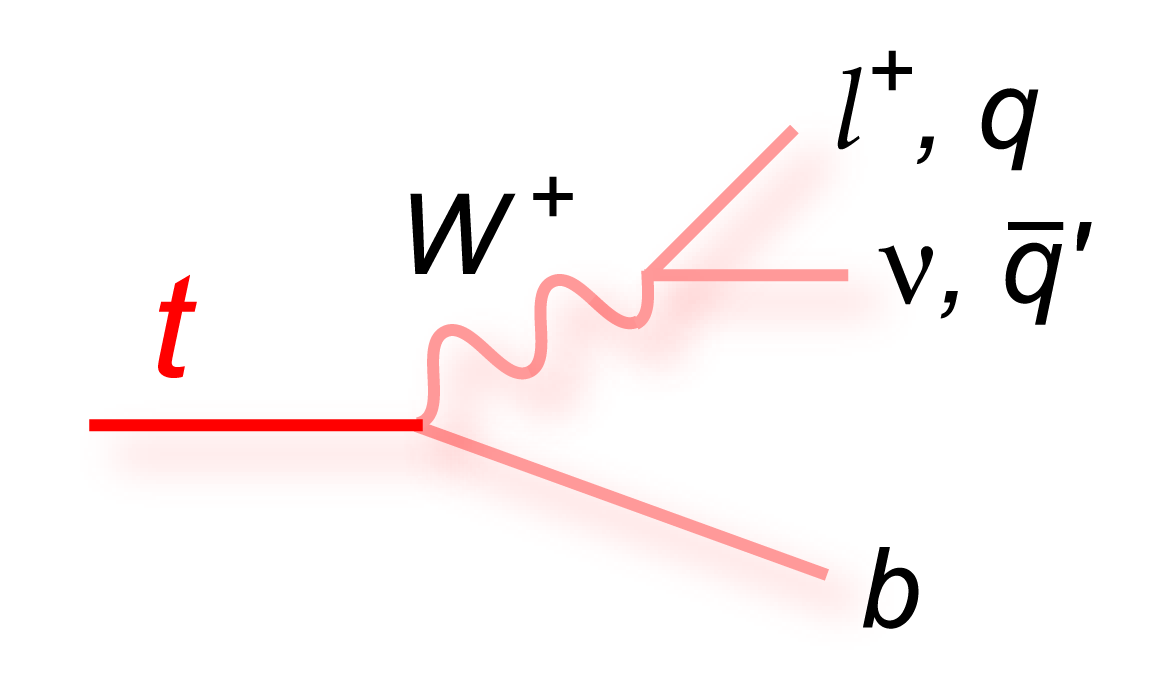
\includegraphics[width=0.49\textwidth]{images/Theory/topdecay.png}
    \caption{Top quark decay to a W boson and b-quark with subsequent decay of the W boson either leptonically or hadronically~\cite{tdecaysource}.}
    \label{fig:tdecay}
\end{center}
\end{figure}

The top quark has the largest Yukawa coupling to the Higgs boson which is of the order of unity. The value of the top quark Yukawa coupling is important in calculations of the stability of the universe and of the energy scales where new physics may arise~\cite{Bezrukov:2014ina}.

\subsection{Top quark pair production}

The first observations of top quarks were made on analyses of top pair production (\ttbar) as this is the dominant mechanism for producing top quarks at colliders. Figure~\ref{fig:ttproduction} shows the leading order tree-level production mechanisms via gluon fusion and quark-anti-quark annihilation. 
%The Feynman rules can be used to calculate the amplitude for each diagram and the summation of the amplitudes gives the theoretical cross section at leading order. 

\begin{figure}[ht!]
\begin{center}
    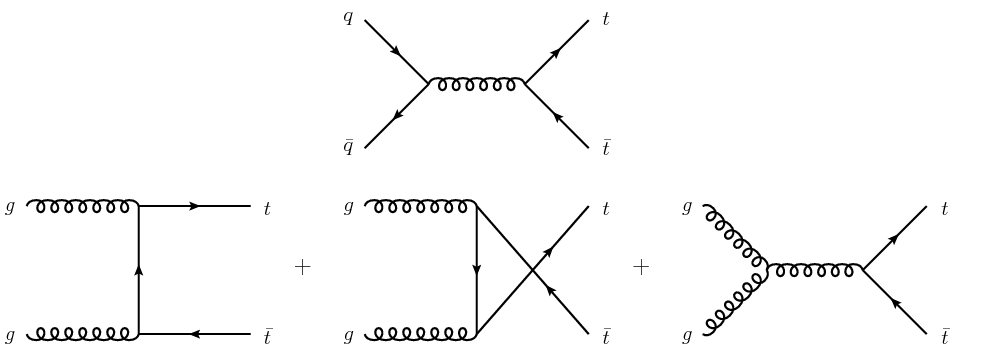
\includegraphics[width=0.95\textwidth]{images/Theory/ttbarfeynman.png}
    \caption{Representative diagrams of top quark pair production in the SM by quark-anti-quark annihilation (top) and via gluon fusion (bottom) at leading order~\cite{Kohn:2012ksa}.}
    \label{fig:ttproduction}
\end{center}
\end{figure}

There are three possible decay modes depending on how each top quark decays, as shown in Fig.~\ref{fig:tdecay}: \emph{hadronic} where both W bosons from the top decay to a quark and anti-quark, \emph{semi-leptonic} where one W boson decays to \qqbar' and one W boson decays to a lepton and a neutrino, and \emph{dileptonic} where both W bosons decay to a lepton and a neutrino each.


\subsection{Single top quark production}

Single top quark production is much rarer than \ttbar production in the SM. It can occur via \qqbar annihilation, g\cPq~fusion or gluon fusion as shown in Fig.~\ref{fig:stFeyn}. In this figure the s-channel (left), t-channel (middle) and associated production with a W boson, tW-channel, (right) are shown.

\begin{figure}[ht!]
\begin{center}
    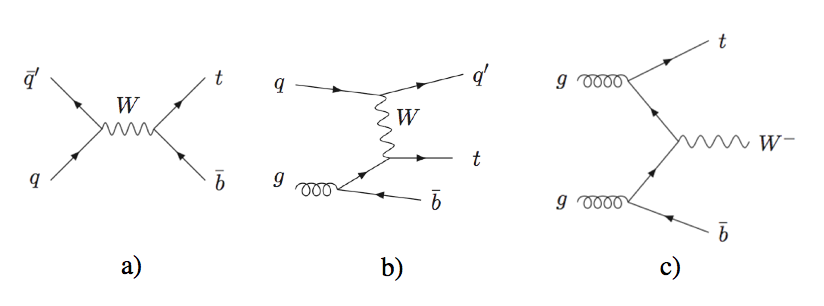
\includegraphics[width=\textwidth]{images/Theory/stFeyn.png}
    \caption{Representative diagrams of single top production at leading order in the a) s-channel , b) t-channel and c) tW-channel~\cite{Lannon:2012fp}.}
    \label{fig:stFeyn}
\end{center}
\end{figure}

The CKM element $|V_{tb}|$ from Eq.~\ref{eqn:CKM2} can be extracted from single top quark decays and the spin of the top quark can be ascertained by studying the leptonic decay of the single top as the charged lepton will point along the direction of the top spin~\cite{Boos:2012hi}.

\subsection{Four top quark production}

The production of four top quarks (\tttt) occurs predominantly via gluon fusion, as seen at leading order in Fig.~\ref{fig:ttttAtLO}, with a $10\%$ contribution from quark-anti-quark annihilation. The production mechanism occurs predominantly via QCD, with smaller contributions from electroweak and Higgs boson mediated terms.


% \begin{figure}[ht!]
% \begin{center}
%     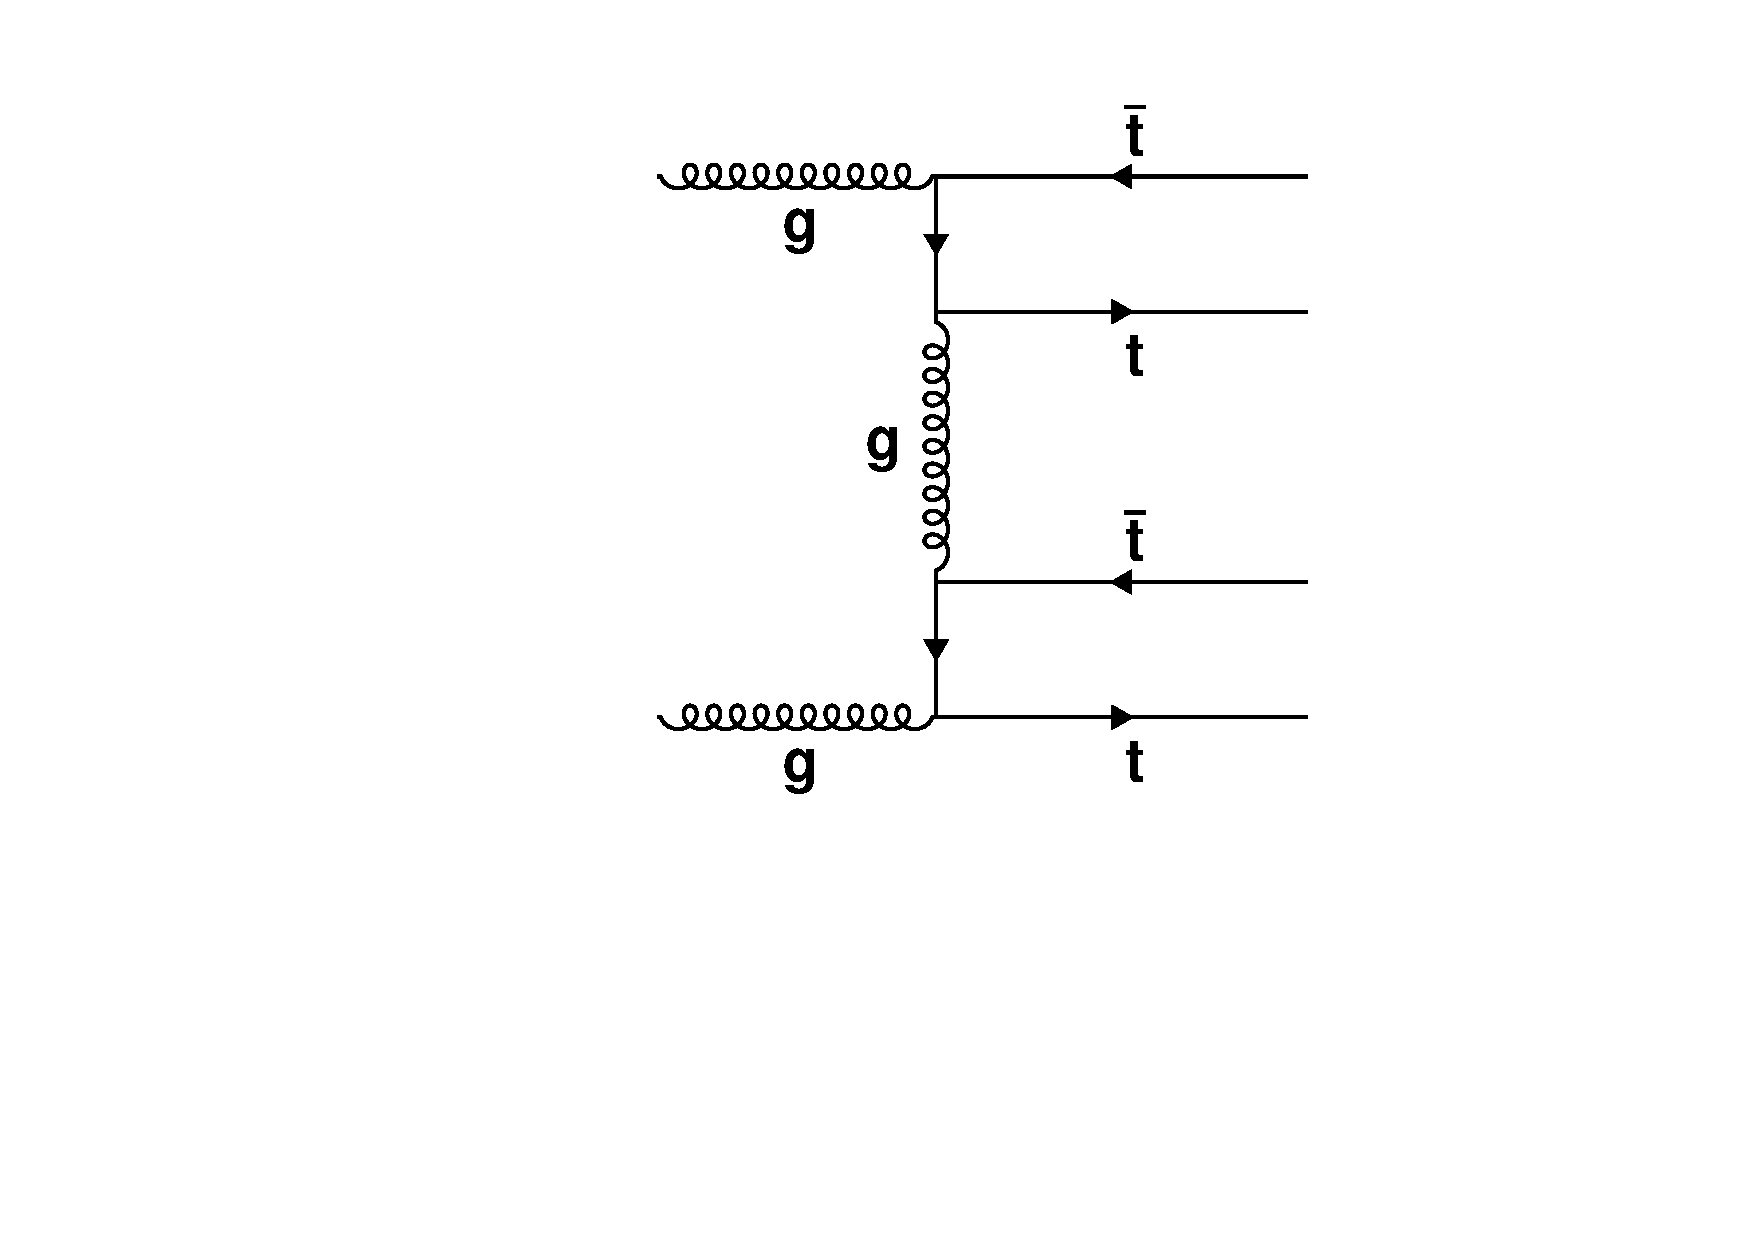
\includegraphics[width=0.49\textwidth]{images/Theory/tttt_t_LO.pdf}
%     \caption{Representative diagram of the production mechanism of \tttt in the SM at LO.}
%     \label{fig:ttttAtLO}
% \end{center}
% \end{figure}

% \begin{figure}[ht!]
% \begin{center}
%         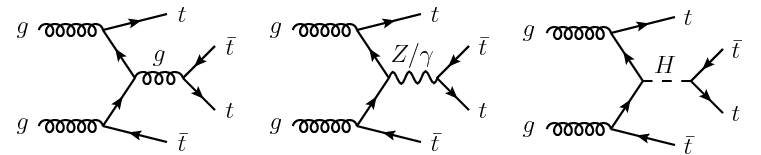
\includegraphics[width=0.7\textwidth]{images/Theory/tttt_feyn_X.png}

%     \caption{Representative diagram of the production mechanism of \tttt in the SM at LO.}
%     \label{fig:ttttAtLO2}
% \end{center}
% \end{figure}


\begin{figure}[ht!]
\begin{center}
    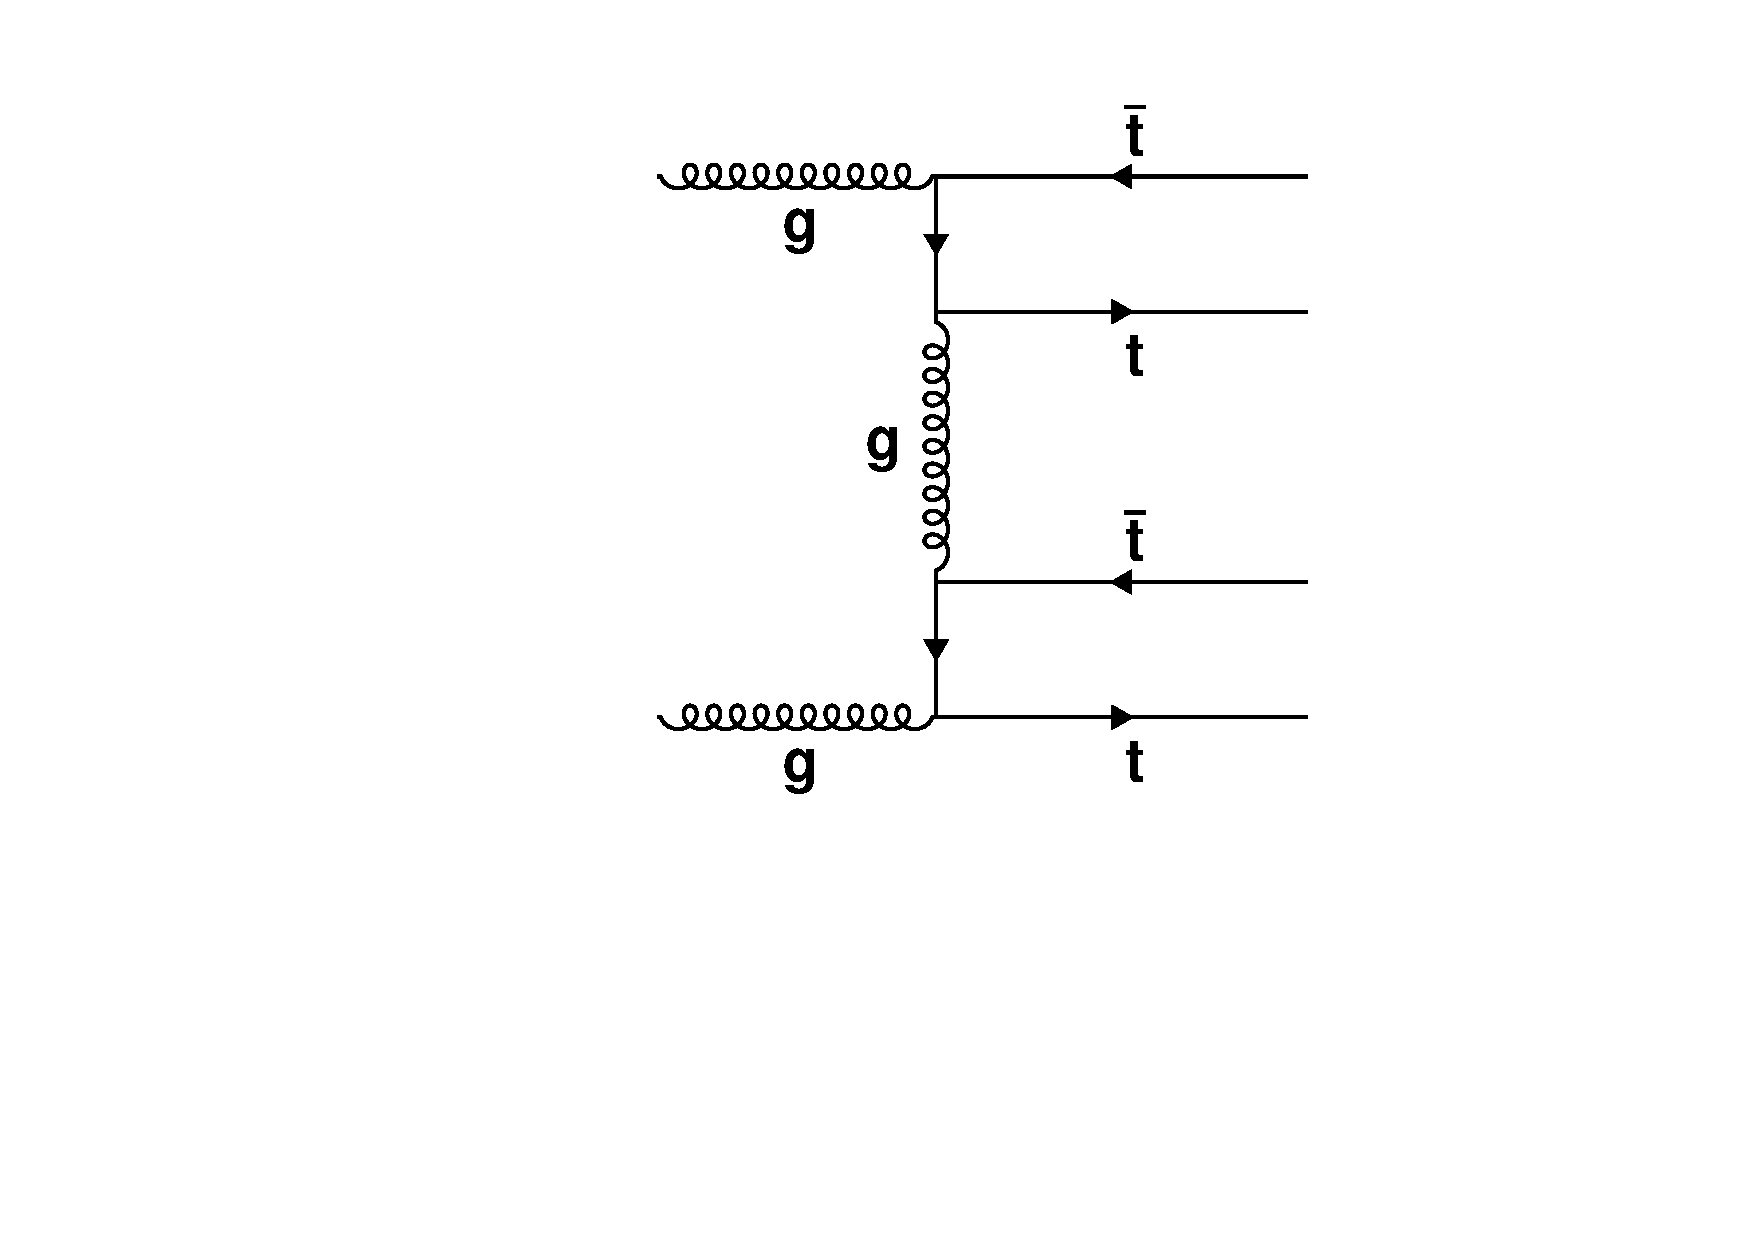
\includegraphics[width=0.2\textwidth]{images/Theory/tttt_t_LO.pdf}
        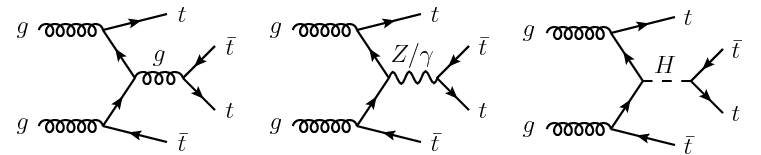
\includegraphics[width=0.79\textwidth]{images/Theory/tttt_feyn_X.png}

    \caption{Representative diagrams of \tttt production in the SM at LO~\cite{Cao:2016wib}.}
    \label{fig:ttttAtLO}
\end{center}
\end{figure}
Higgs boson mediated four top production, as seen in Fig.~\ref{fig:ttttAtLO} (right), is interesting as the cross section is proportional to the fourth power of the top quark Yukawa coupling. Hence, limits can be set on the top quark Yukawa coupling using limits placed on four-top-quark production. The Higgs mediated process can have notable interference with the other terms of O(10\%)~\cite{Cao:2016wib}.
Final states are determined upon whether the weak decay of the W bosons occurs leptonically or hadronically. 

\section{Shortcomings in the standard model ~\label{sec:SMprobs}}
The SM has been resilient to many tests at the LHC and previous collider experiments. However there are many questions about the universe which the SM cannot answer, for instance:\\
{\bf Gravity :} How can gravity be integrated into the SM and is there an associated boson for the gravitational force~\cite{PhysRevLett.107.171101,PhysRevD.82.122001}? \\
{\bf Matter-anti-matter asymmetry :} How did the matter-anti-matter asymmetry in the universe arise when the amount of CP-violation in the SM is not sufficient to account for it~\cite{RevModPhys.76.1}?\\
{\bf Hierarchy problem :} 
The SM does not provide a solution as to why the gravitational force is so much weaker than the other forces. The gravitational coupling constant is O($10^{42}$) smaller than the fine structure constant. Alternatively, one can consider how the masses of weak gauge bosons are O($10^{16}$) smaller than the Planck Mass. The masses of the weak gauge bosons are determined by the Higgs VEV which lies at the relatively small but non-zero value of 246~GeV. The quadratic divergences in the SM calculation of the Higgs VEV suggest that the Higgs field is unstable and should be either zero or at the Planck Energy, ie. O($10^{16}$) larger than it is. The Higgs VEV is considered the be \emph{unnatural} and requires ``fine tuning''~\cite{PhysRevD.20.2619}.\\
% The SM does not provide a solution as to why the Higgs mass is so much smaller than the Planck mass. It also does not describe why the quarks and lepton masses have values which span many orders of magnitude.\\
{\bf Neutrino mass :}
The Sudbury Neutrino Observatory (SNO) observed that the flux of electron neutrinos from the sun was $\approx 1/3$ what it was expected to be~\cite{PhysRevC.88.025501}. This can be explained by neutrino oscillations - $\frac{2}{3}$ of the neutrinos which originated from the nuclear reaction in the sun oscillated into muon and tau neutrinos before reaching the Earth. This means that their mass basis is rotated from their weak-flavour basis and hence neutrinos must have mass, which is not part of the SM.\\
{\bf Dark matter :} Observations of the universe show there is non-baryonic, non-luminous matter which is not accounted for within the SM~\cite{RubinFord}. Studies of galaxy rotation curves show that the angular velocity is relatively constant as a function radius when it should decrease, meaning that there is additional dark matter providing a contribution to the mass of galaxies~\cite{Volders,
Jog:2002dg,
Persic:1995ru}. The presence of dark matter can also be inferred by gravitational lensing. The light from distant stars in the background is curved around the strong gravitational presence of a dark matter cloud, which itself cannot be seen~\cite{Einstein,Ellis2010}. 
This can cause arcs of light and repeated patterns of the same galaxy as seen in Fig~\ref{fig:Glens}.
\begin{figure}[ht!]
\centering
    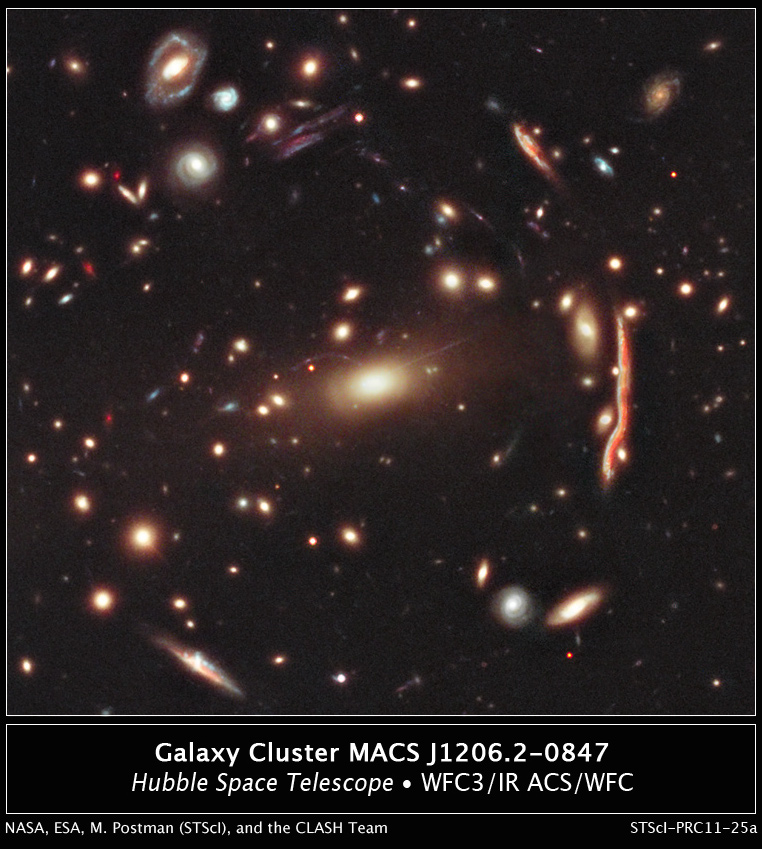
\includegraphics[width=0.65\textwidth]{images/Theory/lensing2.jpg}
    \caption{Gravitational lensing around MACS 1206 as captured by the Hubble Space Telescope~\cite{Glens}.}
    \label{fig:Glens}
\end{figure}


\section{BSM models with four top quark signatures ~\label{sec:BSMmodels}}

There are many theories which try to solve some or all of the problems listed in Section~\ref{sec:SMprobs}. Some theories take a simplified approach rather than using a full Ultraviolet Complete model. These approaches include using an Effective Field Theory (EFT) or Simplified Model, as discussed below.

\subsection{Effective field theories}

An effective field theory can be used in the low-energy limit of a more complete underlying theory. It is used to make observations on final state particles without assumptions on the intermediate particles involved. One example of this is Fermi's theory of beta decay, which was studied before the W boson was discovered. The intermediate W boson particle is replaced with a four-point interaction, as shown in Fig.~\ref{fig:eft1}. Effective field theories work best when there is a large separation between the energy scale being probed and the energy scale of new physics. In the case of the Fermi interaction, the separation between these two scales was three orders of magnitude when it was first studied, and hence it was a valid approximation. 
% (at an energy scale of 10~MeV compared to the mass of the W boson at 80.4~GeV)
\begin{figure}[ht!]
\centering
    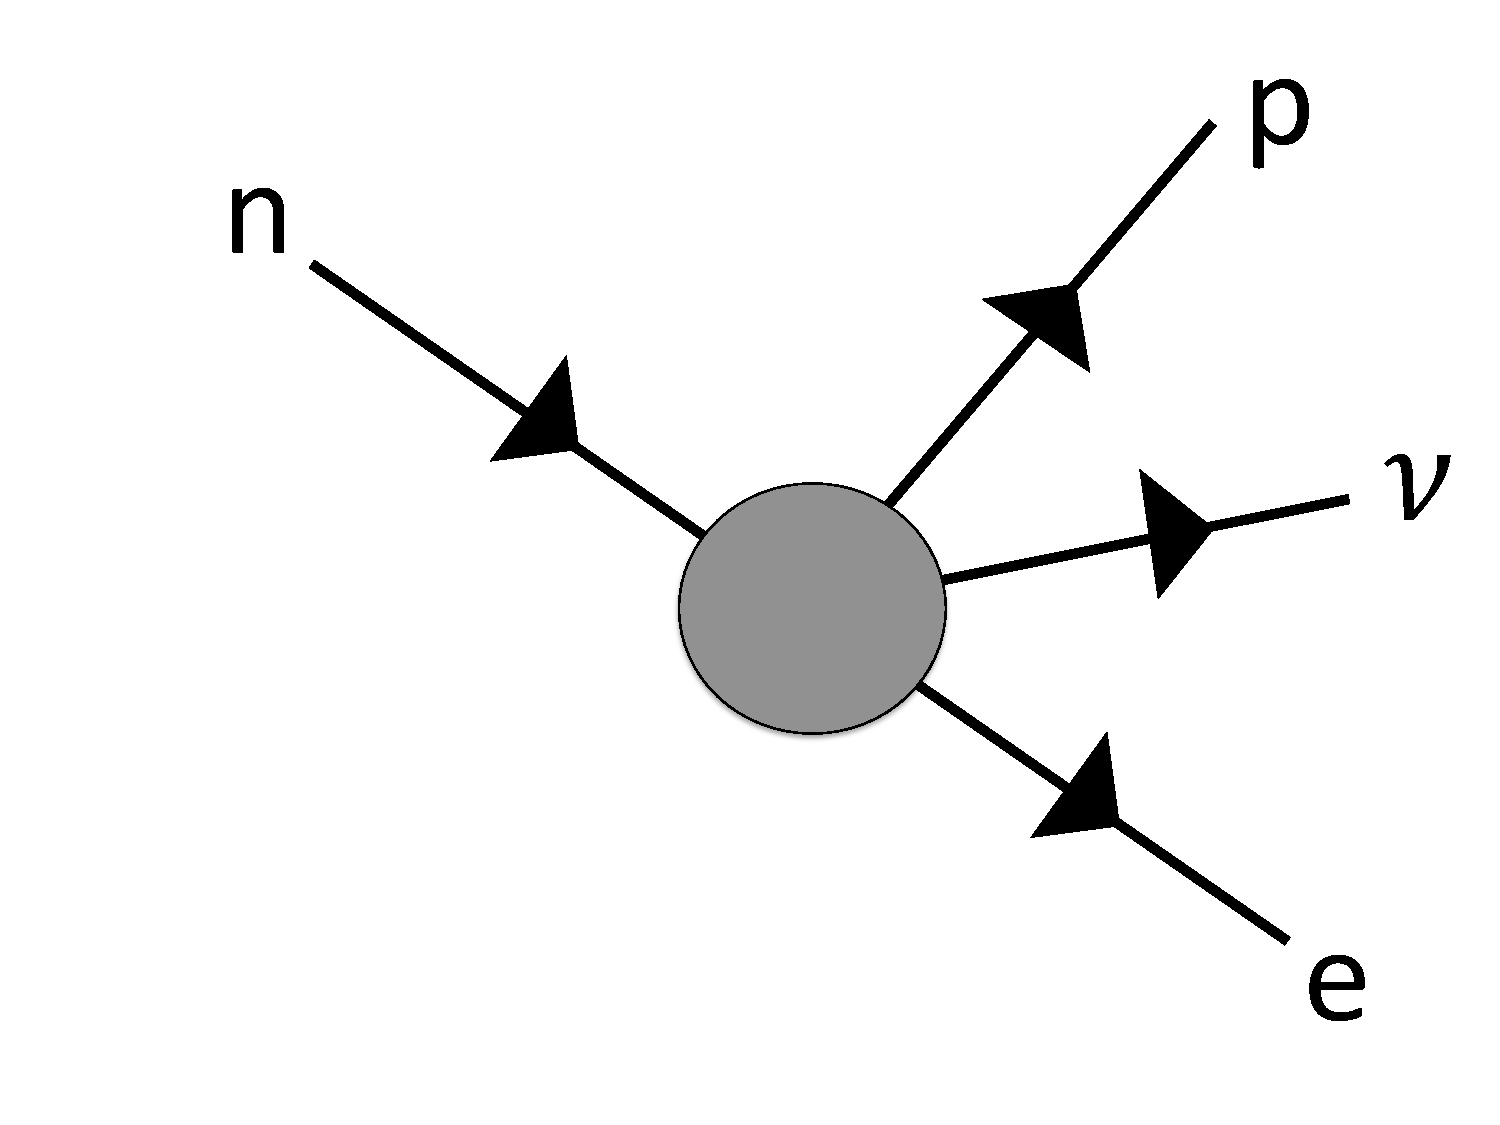
\includegraphics[width=0.45\textwidth]{images/Theory/betadecay.pdf}
    \caption{Fermi interaction for beta decay in an EFT.}
    \label{fig:eft1}
\end{figure}

\subsection{Simplified models}

Simplified models work by building a TeV-scale effective Lagrangian which describes a minimal number of new particles and their interactions. Hence, variables which can be directly observed by the detector can be studied, for example, particle masses, cross sections and branching ratios for different decay modes. Simplified models can sometimes be considered to be a subset of more general physics models where only a few of the particles are considered. Therefore, a simplified model cannot be considered to be model independent but they can help to identify the bounds of sensitivity for searches~\cite{0954-3899-39-10-105005}. An example of where a simplified model can be used is in the case of $\ttbar+\textrm{X}$, as shown in Fig.~\ref{fig:ttXtt}, where the phenomenology of the resulting particles in the detector can be studied without knowledge of which underlying theory the new scalar particle, X, is coming from. In the limit of a large mediator the simplified model is equivalent to an EFT~\cite{DeSimone:2016fbz}.\\

Some BSM theories which have final states containing four top quarks are discussed below. 

\textbf{Top quark Compositeness}\\
It has been hypothesised that the top quark could be a composite particle made up of subparticles named preons, which are bound by a new confining force. Phenomenological studies have been performed in which an EFT is proposed where only the right-handed top quark is considered to be composite. It is argued that if only $t_{R}$ is composite and no other SM component is, then the four top operator (shown in Fig~\ref{fig:eft2}) will be the most significant component of the EFT lagrangian. This can lead to an enhancement of $\approx 10^3$ to the production of \tttt compared to the SM rate~\cite{Tait2topcomp,Tait1topcomp}.

\begin{figure}[ht!]
\centering
    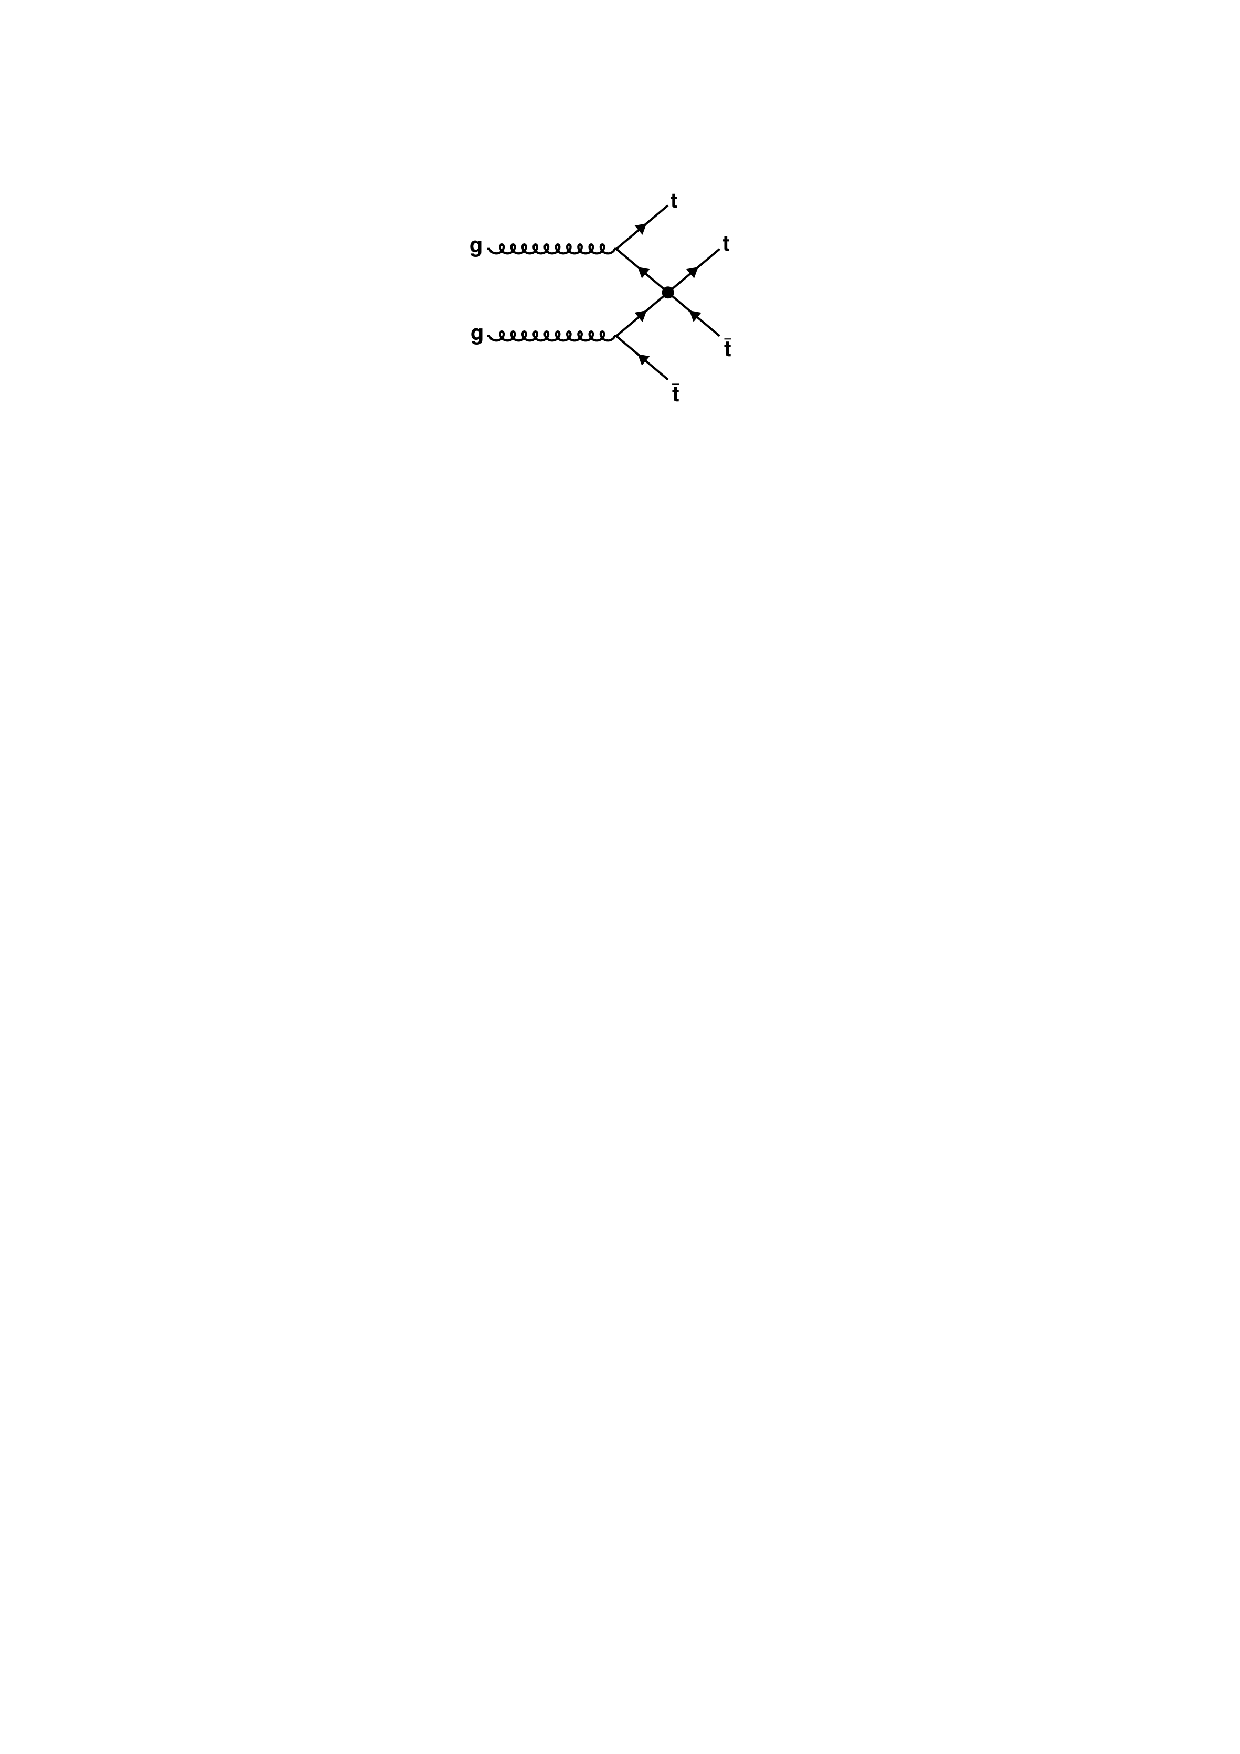
\includegraphics[width=0.45\textwidth]{images/Theory/EFTTopComp.pdf}
    \caption{Four top interaction in an EFT~\cite{Tait2topcomp}.}
    \label{fig:eft2}
\end{figure}

$\boldsymbol{\ttbar+\textrm{X}, ~\textrm{X}}\rightarrow\boldsymbol{\ttbar}$\\
There are several models which contain \ttbar plus an extra scalar particle which then decays to \ttbar as seen in Fig.~\ref{fig:ttXtt}.
The mediator could be a dark matter mediator~\cite{Arina2016}, a heavy Higgs boson~\cite{Bernreuther:2015fts}, or a member of a scalar colour sextet~\cite{Cacciapaglia2015}, for instance. 

\begin{figure}[ht!]
\centering
    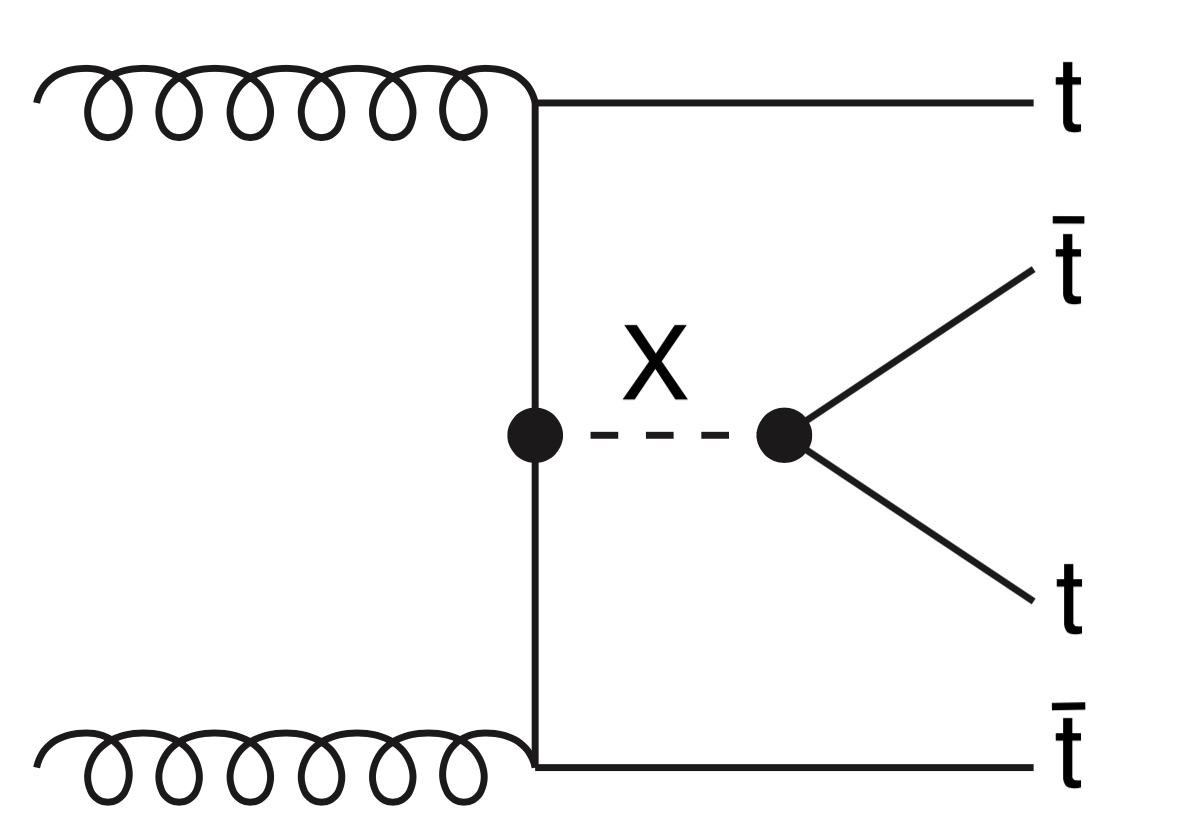
\includegraphics[width=0.45\textwidth]{images/Theory/ttDMtt5.png}
    \caption{Four top production with an intermediate scalar~\cite{Arina2016}.}
    \label{fig:ttXtt}
\end{figure}

% \textbf{Heavy resonances}

\newpage
\textbf{Scalar pair production to $\boldsymbol{\tttt}$}\\
\begin{figure}[ht!]
\centering
    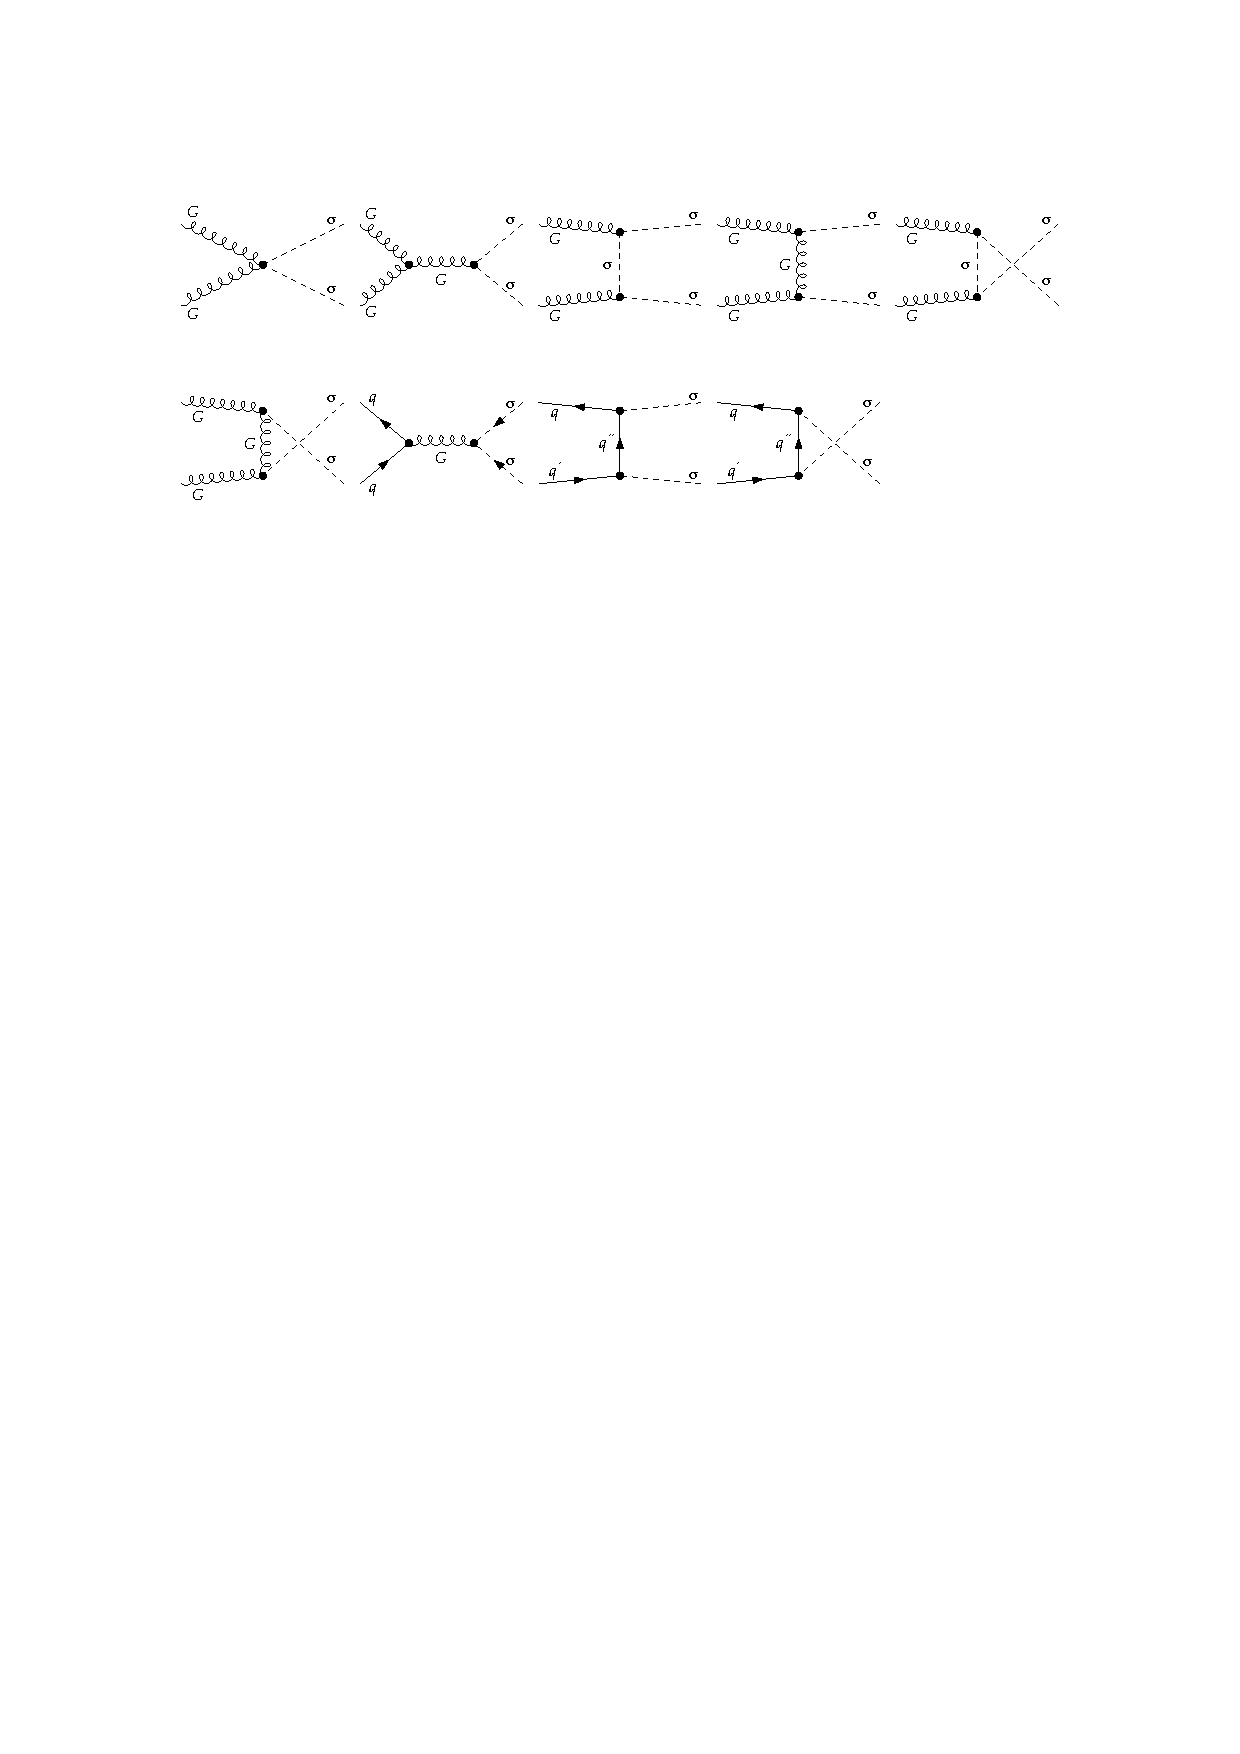
\includegraphics[width=0.99\textwidth]{images/Theory/sgluonFeyn.pdf}
    \caption{Sgluon pair production~\cite{Calvet:2012rk} where G represents gluons and $\sigma$ represents sgluons.}
    \label{fig:sgluonpair}
\end{figure}

An additional scalar gluon (\emph{sgluon}) has been theorised in several models of physics beyond the SM. In N=1/N=2 hybrid~\cite{Fayet:1975yi,AlvarezGaume:1996mv} and R-symmetric~\cite{Salam:1974xa,Fayet:1974pd,Kribs:2007ac} versions of non-minimal supersymmetric models, the minimal supersymmetric model (MSSM) is supplemented by an additional chiral multiplet which lies in the adjoint representation of the QCD gauge group. This supermultiplet contains a two-component fermionic part which mixes with the Dirac gluino and a colour-octet complex scalar particle which is the sgluon field. This is particularly interesting because coloured particles will couple directly to gluons and hence should be produced in proton-proton collisions. Figure~\ref{fig:sgluonpair} shows the possible tree level production modes for sgluon pair production~\cite{Calvet:2012rk}, whilst Fig.~\ref{fig:sgluontttt} shows each sgluon coupling to a \ttbar pair resulting in a final state with four top quarks.
\begin{figure}[ht!]
\begin{center}
    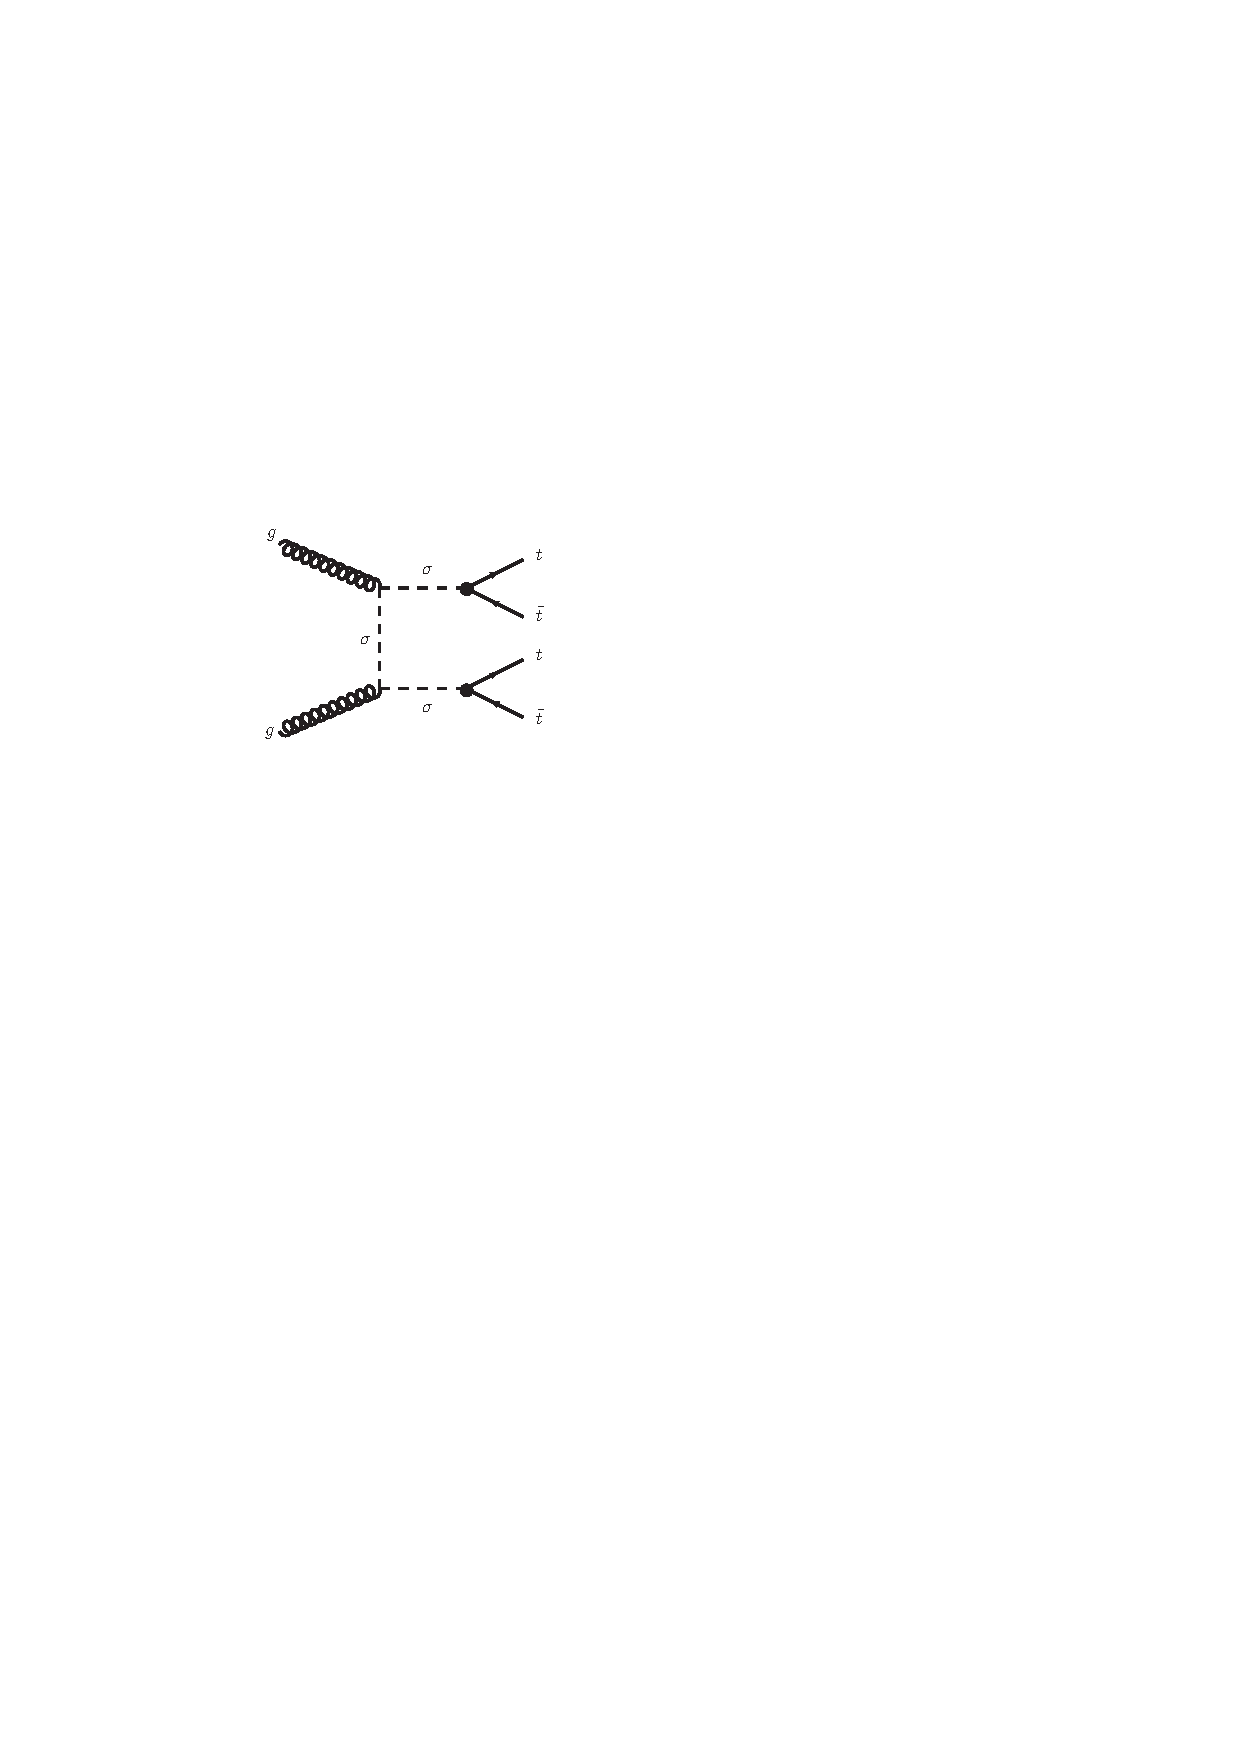
\includegraphics[width=0.4\textwidth]{images/Theory/sgluontotttt.pdf}
    \caption{Representative diagram of sgluon pair production to four-top-quark final state~\cite{Aad:2015kqa}.}
    \label{fig:sgluontttt}
\end{center}
\end{figure}
Sgluons also arise in vector-like confining theories~\cite{Kilic:2009mi} and extra-dimensional models~\cite{Burdman:2006gy}. Therefore it is viable to use a simplified model approach because the final state signatures are reasonably model-independent. Colour octets and sextets can also be pair produced in theories where the Higgs boson is a composite particle~\cite{Cacciapaglia2015}.






